%\documentclass[11pt,a4paper,listof=numbered]{scrreprt}
%\documentclass[11pt,a4paper,listof=numbered]{article}
%\documentclass[9pt,technote]{IEEEtran}
\documentclass[12pt,
titlepage,
a4paper,
oneside,     % ~= twoside
openany,     % keine leeren Seiten
listof=totoc,  % Tab.Abb.verzeichnis
numbers = noenddot, %Keine Punkte hinter Nummerierung der Überschrift
%liststotocnumbered,
%idxtotoc,    % Index
bibliography=totoc,    % Literatur
%bibtotocnumbered,
headsepline, %Linie nach Kopfzeile
]{scrbook} %headsepline 

\usepackage{ifpdf,ifxetex,ifluatex}
\ifpdf % pdflatex
\usepackage[utf8]{inputenc} % Umlaute im Editor direkt
\usepackage[T1]{fontenc} % Wörter mit Umlauten auch sauber trennen, trotz "nicht gefunde" funktioniert es
\usepackage{textcomp} % angeblich outdated, aber benötigt für µ \textmu
\usepackage{lmodern} % Latin Modern, als Schrift gerade in pdfs fluessiger

%\usepackage{ngerman} obsolet, nicht nutzen!
%\usepackage[english]{babel}
\usepackage[ngerman]{babel}
\fi
\ifxetex % xelatex (kompiliert zu xdv, Umwandlung in pdf)
\usepackage{fontspec}
%\usepackage{xltxtra} würde fontspec laden - nicht benötigt
%\usepackage{xunicode} obsolet - ist bereits in fontspec enthalten
%\usepackage{lmodern} funktioniert nicht, aber ist eh Standard für fontspec
\usepackage{polyglossia} % für xelatex besser als babel
\setdefaultlanguage[
babelshorthands = true,
spelling = new
]{german}
%\setotherlanguage[
%variant	= british
%]{english}

\newcommand{\glqq}{„}
\newcommand{\grqq}{“}
\newcommand{\glq}{‚}
\newcommand{\grq}{‘}
\fi

\usepackage{geometry}
%\usepackage{a4wide} durch "geometry" ersetzt
\usepackage{csquotes} %Zitierstil. BibLaTeX erkennt babel und csquotes, und passt sich der Sprache an, (Fallback = AE)
\usepackage[backend       =biber, %oder bibtex 
style         =alphabetic, %or numeric-comp, %3.3.1 Citation Styles
%safeinputenc =false,      %force texencoding=ascii, convert ä->\"{a}
%bibencoding  =utf8,
sorting       =anyt,       %sort by alphabetic label, name, year, title
sortcase      =false,      %dont sort casesensitive
%maxnames     =3           %default for maxbibnames and maxcitenames, ab dem Schwellenwert wird gekürzt
maxbibnames   =316227,     %\printbib -> Kruse et.al.
maxcitenames  =3,          %\cite     -> [Kru+15]
%backref      =true        %list of page numbers, where cited
%backrefstyle =three,      %[3][4][5] -> [3-5] -nur für Seiten
sortlocale    =auto,
urldate       =short,
isbn          =false,
url           =true,
doi           =false,
eprint        =false
]{biblatex}

%\usepackage[babel,autostyle=true]{csquotes}
\bibliography{referenzen.bib}

%\usepackage{bold-extra}  %für \textbf{...} und \textsc{...} bzw. {\bfseries ...} und {\scshape ...} gleichzeitig
\usepackage{dsfont}      %für Zahlenmengen $\mathds{N}\mathds{R}$
%\usepackage{siunitx}    %für si-Einheiten, Leerzeichen und %\si[per-mode = fraction]{\cancel\metre\per\cancel\kilogram\per\second\tothe{2}}
\usepackage{units}       %fuer Tight spacing + Nice fractions + \unitfrac[10]{m}{s}
\usepackage{amsmath}     %erweiterter Formelsatz
\usepackage{amssymb}     %Sonderzeichen für Mathematikmodus
\DeclareMathOperator{\sign}{sign}
\usepackage{ziffer}      %intelgentes Leerz. nach Komma (3,1415 <-> f(x, y))
\usepackage{xspace}      %setzt intelgentes Leerzeichen außer vor.,, und)
\usepackage{nameref}     %für Kapitelnamen bei \nameref auf label
\usepackage{paralist}    %für compactitem mit kleineren Absätzen
\usepackage{pgf,tikz}    %tikz
\usepackage{mathrsfs} 	 %tikz
\usetikzlibrary{arrows}  %tikz
\usepackage{graphicx}    %Standard Latex Grafiken, svg nach latex
\usepackage{color}       %svg nach latex
\usepackage{transparent} %svg nach latex
\usepackage{import}      %Grafiken in anderem Ordner
\usepackage{caption}     %mehrere Grafiken in einer Abb.
\usepackage{subcaption}  %mehrere Grafiken in einer Abb.
\usepackage{url}         %im Zweifel besser formariere Links
\setcounter{biburlnumpenalty}{100} %erweitern Package url
\setcounter{biburlucpenalty}{100}
\setcounter{biburllcpenalty}{100}
%\usepackage{wrapfig}    %fuer Grafiken im Fließtext

%\usepackage{float}      %ersetzt durch tocbasic (s.u.) %fuer Grafiken im Fließtext, fuer Positionierungsoption [H], welches [h] erzwingt
\usepackage{tocbasic}

%\usepackage{fancyhdr}   %Kopf- und Fußzeile
\usepackage{tabularx}    %Textausrichtung bei fester Spaltenbreite
%https://de.wikibooks.org/wiki/LaTeX-W%C3%B6rterbuch:_tabular
\newcolumntype{L}[1]{>{\raggedright\arraybackslash}p{#1}} % linksbündig mit Breitenangabe
\newcolumntype{C}[1]{>{\centering\arraybackslash}p{#1}} % zentriert mit Breitenangabe
\newcolumntype{R}[1]{>{\raggedleft\arraybackslash}p{#1}} % rechtsbündig mit Breitenangabe

\usepackage{longtable}
%\usepackage{tabu}
\usepackage{booktabs}	%für schickere Tabellen, darunter top-, mid-, bottomrule und z.B. \cmidrule(r){1-2}
\usepackage{multicol}	%Tabellen mit Zelle über mehrere Spalten
\usepackage{multirow}	%Tabellen mit Zelle über mehrere Zeilen

\usepackage{pdfpages} %einfügen von PDF-Dokumenten

\usepackage[onehalfspacing]{setspace} %Zeilenabstand

\usepackage{suffix}
\usepackage{xstring}

%Paketdoku lesen lohnt sich für nette Optionen
\usepackage[%hyperref, % Kurzformen verlinken auf die \printacronyms % bekannter Fehler: https://bitbucket.org/cgnieder/acro/issues/76/hyperref-option-does-not-work-with-xelatex
%single, % bei einmaligem \ac wird kein Eintrag erstellt
%tooltip, % erzeugt ein tooltop
%list-style = longtable, % Listenart
%list-heading = chapter % Überschriftart
]{acro}
\acsetup{make-links=true}
\acsetup{list/display=used}
\acsetup{list/template=longtable}
\acsetup{list/heading=chapter}
%\ExplSyntaxOn % _ and : are valid characters for function names until \ExplSyntaxOff


\DeclareAcronym{imn}{
	short		= \textit{IMN} ,
	long		= \textit{Institut für mobile Maschinen und Nutzfahrzeuge},
	short-plural= s,
	long-plural	= s
}
\DeclareAcronym{catiaV5}{
	short		= \textit{CATIA V5} ,
	long		= \textit{Computer Aided Three-Dimensional Interactive Application V5} ,
	extra		= CAD-System der Dassault Systèmes SE % erscheint nur in \printacronyms %AblaufValidierung o.Ä. ergänzen (nur für die Liste)
}
\DeclareAcronym{yolo}{
	short		= \textit{YOLO} ,
	long		= \textit{You Only Look Once} ,
	extra		= Man schaut nur einmal hin
} % müssen in Präambel deklariert werden 


%hyperref immer als letztes einbinden!
\usepackage[bookmarksopen = true, %öffnet Struktur bei Adobe
colorlinks    = true, %keine Rahmen
linkcolor     = black, %für \ref
citecolor     = black,
urlcolor      = black,
german
]{hyperref} %fuer Hyperlinks bei refs und sections

\newcommand{\ve}[1]{\ensuremath \boldsymbol{#1}\xspace}
\newcommand{\varTitel}{Bewertung von KI-Algorithmen zur luftgestützten Objekt-Detektion in landwirtschaftlichen Umgebungen}
\newcommand{\varAuthor}{Henrik Bullinger}
\newcommand{\scFt}{\textsc{Fourier}-Transformation\xspace}

%opening
\title{\varTitel}
\date{\today}
\author{\varAuthor}
%\dedication{Widmung}

\begin{document}
\frontmatter
\pagenumbering{Roman}

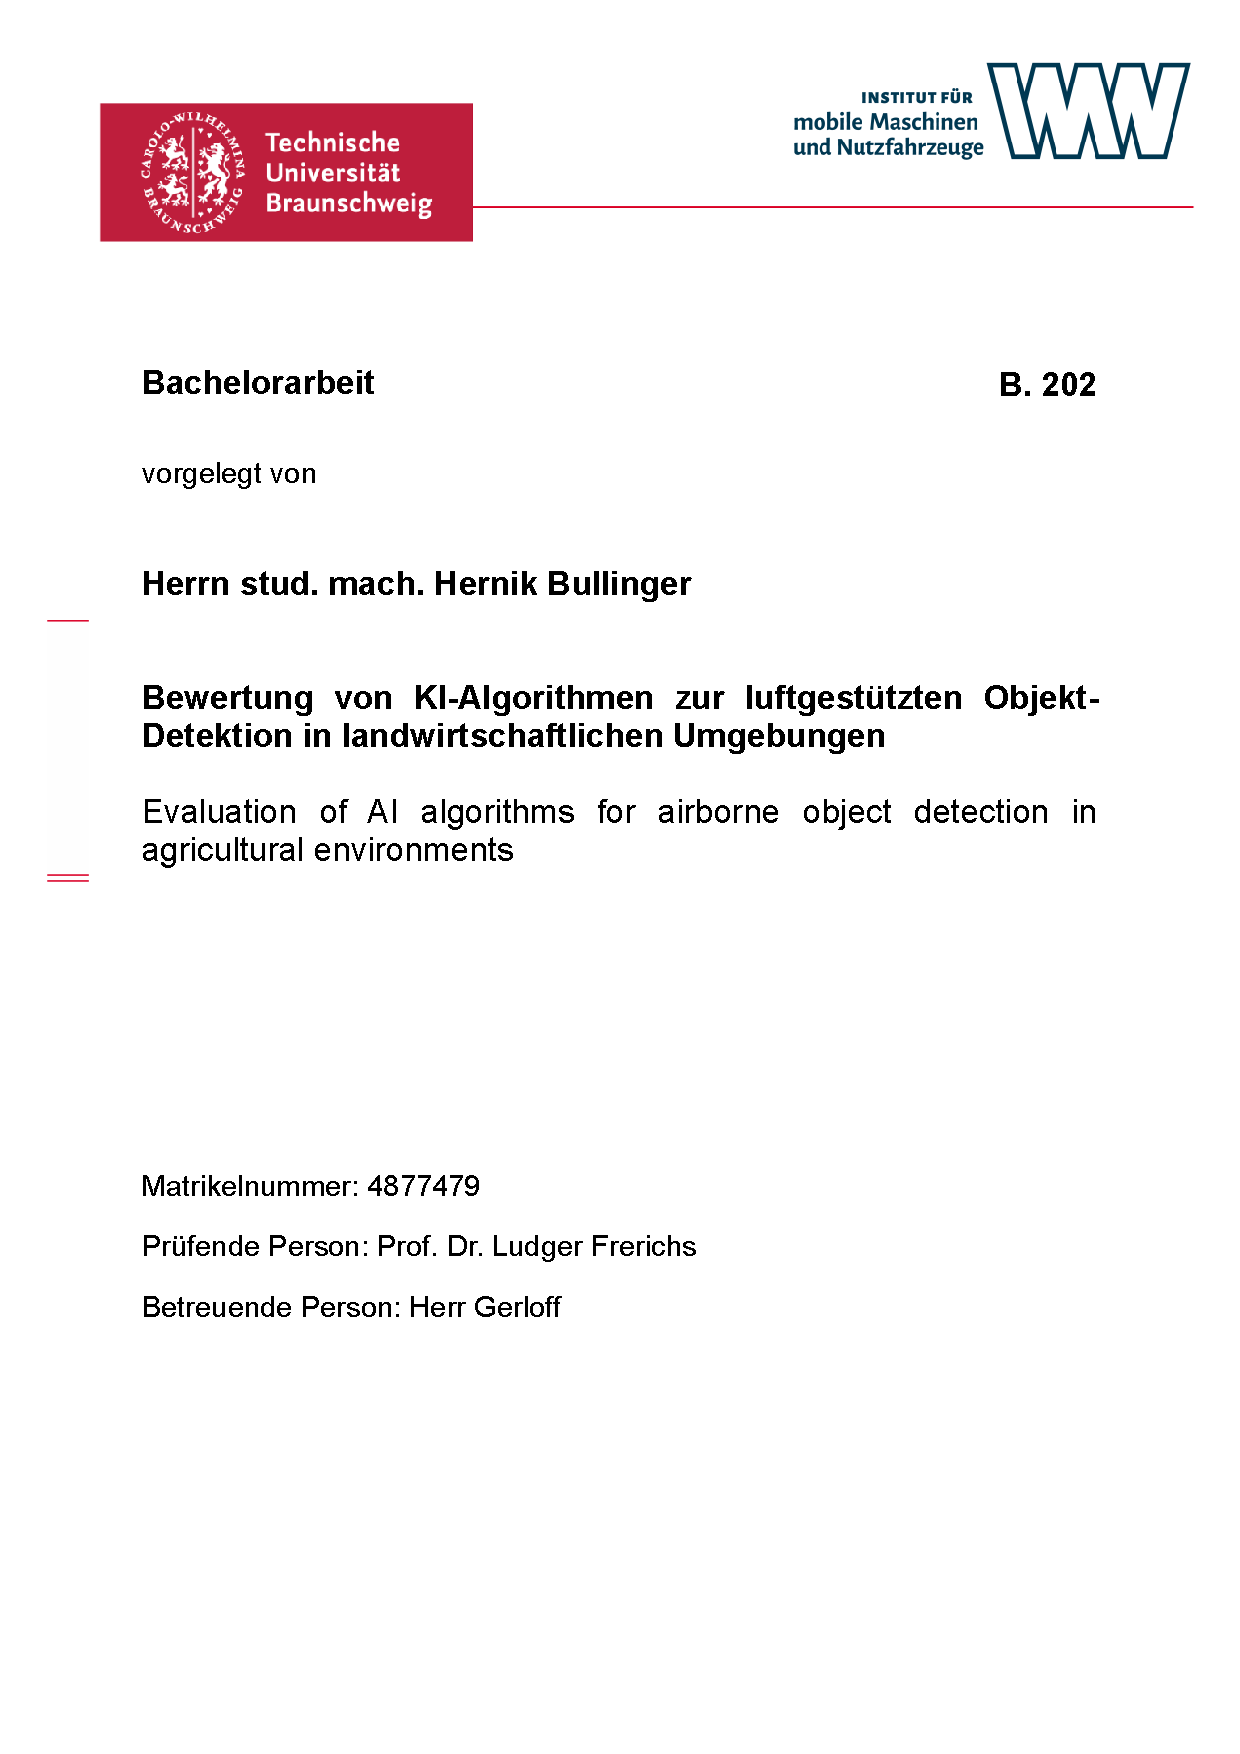
\includepdf[pages=-]{Bullinger_Deckblatt}

\section*{Sperrvermerk}
Wird bei Bedarf eingefügt! \\
Vorgabe erfolgt durch das Institut IMN

\newpage
\section*{Selbstständigkeitserklärung}
Hiermit versichere ich, dass ich die vorliegende Arbeit selbstständig verfasst habe, keine anderen als die angegebenen Quellen und Hilfsmittel benutzt wurden, alle Stellen der Arbeit, die wörtlich oder sinngemäß aus anderen Quellen übernommen wurden, als solche kenntlich gemacht sind, und die Arbeit in gleicher oder ähnlicher Form noch keiner Prüfungsbehörde vorgelegen hat. \\
\\
Braunschweig, den 18. Januar 2023 \\
\\
\\
Henrik Bullinger \\



\listoffigures

\listoftables

\printacronyms

\newpage
\chapter*{Abstract}
Kurze Erläuterung der Neuerungen:\\
maximal eine Seite, i.d.R. in englischer Sprache verfasst

\newpage
\tableofcontents

\mainmatter
\chapter{Einleitung}
\label{cha:einleitung}

Durch eine stetig anwachsende Weltbevölkerung und aufgrund des anthropogenen Klimawandels steigen die Anforderungen an die Landwirtschaft. Die Bewirtschaftung von schrumpfenden landwirtschaftlichen Flächen muss effizienter gestaltet werden, damit die Versorgung aufrecht erhalten werden kann. Durch eine Umstellung auf nachhaltige und ressourcenschonende landwirtschaftliche Betriebe, kann die Herausforderung bewerkstelligt werden. Ein grundlegender Schritt ist hierbei der Einsatz von autonomen Maschinen, welche mittels Künstlicher Intelligenz betrieben werden. \\
Insbesondere Drohnen dienen hierbei der Überwachung aus der Luft, sowohl zum Wohl der Pflanzen, als auch zur Erkennung von Gefahren für Mensch und Tier. Um diese Dinge zu erkennen werden Algorithmen zur Objekterkennung verwendet, welche im Folgendem auf ihre Eignung in der landwirtschaftlichen Umgebung geprüft werden.

\chapter{Stand der Technik}
\label{cha:sdT}

\section{Landwirtschaft}
\label{sec_landwirtschaft}

\subsection{ISO Barrel 18497}
\label{subsec_iso}

Die \ac{iso} Norm 18497 beschreibt die Sicherheitsanforderungen an autonome Maschinen im Feldeinsatz in der Landwirtschaft. In ihr ist ein standardisiertes Hindernis definiert, welches als \ac{iso} Barrel 18497 gekennzeichnet ist und von dem Algorithmus erkannt werden muss. In Abbildung \ref{fig:isoBarrel} sind die genauen Maße dieses Objekts dargestellt. \\

\begin{figure}[h]
	\centering
	\def\svgwidth{0.6\columnwidth}
	\import{Abbildungen/}{isoBarrel_Maße.pdf_tex}
	\caption{Maße des \ac{iso} Barrel 18497}
	\label{fig:isoBarrel}
\end{figure}

Um den Härtefall im landwirtschaftlichen Betrieb darzustellen wird das \ac{iso} Barrel grün angemalt. Das beruht auf dem Hintergedanken, dass die landwirtschaftliche Umgebung ebenfalls meist grün ist und es somit dem Algorithmus schwer gemacht werden soll das \ac{iso} Barrel als solches zu erkennen. Abbildung \ref{fig:isoBarrelBsp} zeigt beispielhaft den angesprochenen Fall im Feldeinsatz. \\

\begin{figure}[h]
	\centering
	\def\svgwidth{0.8\columnwidth}
	\import{Abbildungen/}{isoBarrel_Bsp.pdf_tex}
	\caption{Rot umrandetes \ac{iso} Barrel 18497 inmitten Gräser}
	\label{fig:isoBarrelBsp}
\end{figure}

Die Erkennbarkeit dieses Objektes stellt somit die grundlegende Bedingung der zu bewertenden Algorithmen aus Kapitel \ref{cha:algorithmen} dar.

\section{Sensorik}
\label{sec_sensorik}

Zum Einsatz bei der Objekterkennung mittels Algorithmen werden meist \ac{lidar}- und \ac{rgb}-Sensoren, sowie auch Multispektralkameras verwendet. Wobei letztere eher selten zum Einsatz kommen.

\section{Künstliche Intelligenz}
\label{sec_ki}

\subsection{Machine Learning}
\label{subsec_machine}

\subsection{Deep Learning}
\label{subsec_deep}

\subsection{Convolutional Neural Network}
\label{subsec_cnn}



\chapter{Algorithmen}
\label{cha:algorithmen}



\section{YOLO-Algorithmus}
\label{sec_yolo}

\section{R-CNN-Algorithmen}
\label{sec_rcnnalg}

\subsection{R-CNN}
\label{subsec_rcnn}

\subsection{Fast R-CNN}
\label{subsec_frcnn}

\subsection{Faster R-CNN}
\label{subsec_ffrcnn}

\subsection{Mask R-CNN}
\label{subsec_mrcnn}

\section{Single shot Detection}
\label{sec_ssd}



\chapter{Bewertungskriterien}
\label{cha:bewertungskriterien} 



\section{Detektionsgeschwindigkeit}
\label{sec_detgeschw}

\section{Detektionsgenauigkeit}
\label{sec_detgenau}

\section{Speicherplatz}
\label{sec_speicher}

\section{Fehleranfälligkeit}
\label{sec_fehler}


\chapter{Auswertung der Kriterien}
\label{cha:auswertung}



\chapter{Fazit}
\label{cha:fazit}



\section{Citation}
\label{sec_citation}

The citation is the foundation of scientific work. This template uses a .bib library which is included as \textbf{referenzen.bib} in the header. You can see the file in the directory. I recommend \textit{CITAVI} for Literature collection.
In the \textbf{.bib} every entry has its unique name, e.g. \textbf{Winner.2017b}. Cite with the commant \cite{Winner.2017b}
The .bib can contain unused entries which wont be plotted in the bibliography.

\section{Acronyms}
\label{sec_acronyms}

First use of acronyms are the declaration \ac{catiaV5}.  \\
second use is short \ac{catiaV5} \\
If you declare a acronym but use it only once, it will only be the long form without short declaration. \ac{imn} 

\ac{imn} and the german Genitiv des \acp{imn}

\section{Equations}
\label{sec_Equations}

Some fancy special math textlayouts \scFt.

Die Kraft~$\ve{F} = \nicefrac{P}{v}$ berechnet sich zu

And Equations with automated numbering
\begin{align}
	F &= m \cdot a = 0,5 \nonumber\\
	&= \left( \frac{1}{\frac{4}{2}} + 1 \right)	\label{gl:Fdef}\\
	&\neq 7 \int_{x=0}^{7} x \, \mathrm{d}x ~ \epsilon \varepsilon \phi \varphi
\end{align}

Gemäß~\ref{gl:Fdef} gilt

\section{Tables}
\label{sec:tables}

The placement of the tables follows the same rules as described for the figures before

\begin{table}[h]
	\caption{Tabellenüberschrift}
	\label{tab_ExampleTable}
	\centering
	\begin{tabular}{l l r}
		Fahrzeug & Name & Wert \\
		\toprule
		Auto & Peter & 3  \\ 
		Pferd & Hans & 5  \\
	\end{tabular}
\end{table}

\section{Figures}
\label{sec_figures}

Connected Figures, see \ref{fig:leck_toll}
\begin{figure}
	\centering
	\begin{subfigure}[b]{0.48\textwidth}
		\def\svgwidth{\columnwidth}
		\import{AbbEinleitung/}{peter.pdf_tex}
		\caption{Zeitbereich}
		\label{leck_toll_t}
	\end{subfigure}
	~
	\begin{subfigure}[b]{0.48\textwidth}
		\def\svgwidth{\columnwidth}
		\import{AbbEinleitung/}{peter.pdf_tex}
		\caption{Bildbereich}
		\label{leck_toll_f}
	\end{subfigure}
	\caption{Abgetastetes Signal ohne Leckeffekt. Bsp. mit $N$=10; $F_s$=\unit[1]{kHz}; $T_s$=\unit[10]{ms}}
	\label{fig:leck_toll}
\end{figure}


\printbibliography

\label{letzteSeite}
\appendix

\chapter{Anhang}
\label{cha_ausb}
\pagenumbering{roman}

\section{Leitfaden zur Erstellung studentischer Arbeiten am IMN}
\label{sec_Leitfaden}

\includepdf[pages=-]{Leitfaden-Erstellung-studentischer-Arbeiten-IMN_Version-3.1}

\end{document}
